\documentclass[conference]{IEEEtran}
\usepackage{cite}
\usepackage{amsmath,amssymb,amsfonts}
\usepackage{algorithmic}
\usepackage{graphicx}
\usepackage{textcomp}
\usepackage{xcolor}
\usepackage{booktabs}
\usepackage{tikz}
\usepackage{pgfplots}
\usepackage[T1]{fontenc}
\pgfplotsset{compat=1.17}
\usetikzlibrary{positioning, arrows.meta, shapes.geometric}
\usepackage{hyperref}

\def\BibTeX{{\rm B\kern-.05em{\sc i\kern-.025em b}\kern-.08em
    T\kern-.1667em\lower.7ex\hbox{E}\kern-.125emX}}

\begin{document}

\title{Canon-Aware Retrieval: User-Determined Provenance Arbitration in Parallel-Valid Fiction Domains}

\author{\IEEEauthorblockN{Sannihith Vikram Javvadi}
\IEEEauthorblockA{\textit{Department of Computer Science \& Engineering} \\
\textit{VNR Vignana Jyothi Institute of Engineering and Technology}\\
Hyderabad, Telangana, India \\
sannihithjavvadi@gmail.com}
}

\maketitle

\footnotetext{Code and benchmark: \url{https://github.com/hvocr/canon-aware-rag}}

\begin{abstract}
Retrieval-Augmented Generation (RAG) systems implicitly assume that retrieved passages are mutually consistent. This assumption fails in domains where multiple authoritative versions of the same fact coexist without a hierarchy --- legal jurisdictions, competing clinical guidelines, historical disputes, and fiction canon. Prior work on conflict-aware RAG resolves such conflicts by selecting a winner (via credibility, temporal scope, or graph consistency) or by adjudicating a stance and abstaining. This work studies \emph{user-determined provenance arbitration}, in which the authoritative source is specified by the user. We release a provenance-annotated benchmark of 43 canon conflicts and 124 evaluation queries across three Stephen King works, with inter-annotator agreement of $\kappa = 0.85$. We evaluate seven retrieval-and-generation configurations and measure both retrieval-level precision and answer-level correctness. The two metrics diverge sharply. A classifier-based variant raises retrieval precision on explicit queries from 0.46 to 0.98 while answer correctness stays flat (0.51 to 0.49). A keyword-filter variant improves retrieval precision but halves answer correctness (0.51 to 0.27). A universal per-branch generation prompt achieves the highest raw correctness scores (0.59 explicit, 0.82 implicit, 0.83 ambiguous). However, because the evaluation judge rewards the correct fact regardless of whether other branches are included, this configuration does not guarantee strict provenance arbitration. In our setting, branch-label retrieval precision does not predict answer-level correctness, and the largest single improvement to ambiguous-query correctness comes from the generation prompt rather than the retrieval method. We report this as an empirical finding from a single-generator, single-run experiment.
\end{abstract}

\begin{IEEEkeywords}
retrieval-augmented generation, knowledge conflict, provenance, source authority, narrative question answering
\end{IEEEkeywords}

\section{Introduction}

Retrieval-Augmented Generation (RAG)~\cite{lewis2020} grounds large language model outputs in external knowledge, reducing hallucination and enabling knowledge-intensive tasks. The core pipeline retrieves relevant passages and conditions generation on them. This pipeline implicitly assumes that retrieved passages are mutually consistent: that if two passages describe the same fact, they agree.

This assumption fails frequently. In legal RAG, jurisdictional branches state contradictory rules. In medical RAG, competing clinical guidelines recommend different treatments. In fact-checking, sources of varying credibility assert incompatible claims. In each case, a system that concatenates retrieved passages will produce an answer that silently merges contradiction.

A growing body of work addresses this. ConflictRAG~\cite{conflictrag} detects and classifies conflicts and resolves them by ranking source credibility. TruthfulRAG~\cite{truthfulrag} resolves conflicts via knowledge graph consistency. T-GRAG~\cite{tgrag} models temporal conflict and applies time-scope matching as a retrieval rule. ConRAG~\cite{conrag} makes conflict explicit through an evidence table but still adjudicates a correct stance and abstains when evidence is balanced. Across these works, conflict is treated as an anomaly to be eliminated --- the system determines which source is authoritative.

We study a domain where this framing is wrong. In fictional canon, multiple versions of the same story are all legitimate. The novel and the film are not competing claims about a single world; they are parallel valid branches. The correct source is determined by what the user asked for, not by credibility, temporal scope, or graph consistency. We call this \emph{user-determined provenance arbitration}.

We make four contributions:
\begin{enumerate}
\item A \textbf{reframing}. We formalize the distinction between system-determined arbitration (prior work) and user-determined arbitration (this work), and identify parallel-valid canon domains as a clean test case for the latter.
\item A \textbf{benchmark}. We release a provenance-annotated corpus of 436 chunks across 11 canon branches, a seed fact table of 43 verified canon conflicts, and 124 evaluation queries across four types (EXPLICIT, IMPLICIT, AMBIGUOUS, CONTROL), with inter-annotator agreement of $\kappa = 0.85$.
\item A \textbf{measurement}. We evaluate seven retrieval-and-generation configurations at both the retrieval level and the answer level. We find that the two metrics diverge sharply: the variant with the highest retrieval precision produces no improvement in answer correctness, and a keyword-filter variant that modestly improves retrieval precision halves answer correctness.
\item A \textbf{measurement of component contribution}. Through an ablation, we separate the retrieval and generation components of branch-aware RAG. In our setting, a per-branch generation prompt accounts for most of the ambiguous-query gain, while per-branch retrieval adds one additional correct answer out of 24 beyond the prompt. We report this from a single-generator, single-run experiment and note that our per-branch prompt and AMBIGUOUS judge both reward covering multiple versions.
\end{enumerate}

\section{Related Work}

\subsection{Conflict-Aware RAG}

\textbf{ConflictRAG}~\cite{conflictrag} addresses inter-document conflicts --- cases where retrieved passages contradict each other. It detects and classifies conflicts before generation, then resolves them by ranking source credibility using an Entropy-TOPSIS framework. The implicit assumption is that when two sources disagree, one is more credible.

\textbf{TruthfulRAG}~\cite{truthfulrag} addresses parametric-contextual conflicts, where retrieved evidence contradicts the model's internal knowledge. It builds a knowledge graph from retrieved content and applies entropy-based filtering to identify and remove conflicting triples. Graph consistency determines truth.

\textbf{T-GRAG}~\cite{tgrag} addresses temporal conflicts. It models knowledge as an evolving graph and retrieves the version appropriate to the query's time scope. The retrieval rule is time-scope matching.

\textbf{ConRAG}~\cite{conrag} makes multi-source disagreement explicit rather than silently merging it. It tags passages as Support, Refute, or Irrelevant, clusters them into consistent evidence groups, and computes a conflict score. When disagreement is high, it preserves both sides and generates an answer with an explicit stance and sentence-level citations. However, ConRAG still adjudicates a correct stance and abstains when evidence is balanced --- it assumes a single ground truth exists even when the system cannot determine it.

\textbf{Authority Bias in RAG}~\cite{authoritybias} studies conflicts between user-provided knowledge and retrieved facts, finding that LLMs over-trust the user and proposing a mitigation framework that favors retrieved facts. The assumption is that user input is a factual claim that can be wrong.

\textbf{MAGIC}~\cite{magic} is a benchmark for detecting and localizing inter-context conflicts. It generates synthetic conflicts by manipulating entities and relations in knowledge graphs. 

\textbf{CONFACT}~\cite{confact} studies fact-checking under conflicting evidence from sources of varying credibility, and shows that incorporating media source credibility improves conflict resolution. Again, the assumption is a credibility hierarchy.

\subsection{Narrative-Aware Retrieval}

\textbf{Narrative Knowledge Weaver (NKW)}~\cite{nkw} recognizes that narrative QA requires reasoning over dynamic character states and causal triggers, and builds a framework aligning textual evidence with canonical graph structure, entity profiles, and storylines. However, NKW assumes a single coherent story world --- its canonical graph presumes consistency within one narrative.

\subsection{The Shared Assumption}

Across all prior works, conflict is treated as an anomaly to be eliminated. Each proposes a mechanism to select a winner: credibility ranking~\cite{conflictrag,confact}, graph consistency~\cite{truthfulrag}, time-scope matching~\cite{tgrag}, coherence within one story world~\cite{nkw}, or factual correctness over user input~\cite{authoritybias}. ConRAG~\cite{conrag} advances the field by making conflict explicit rather than silently merging it, but still adjudicates a stance.

Two assumptions are shared across the field. First, that the system should determine which source is authoritative for a given query. Second, that improvements in retrieval quality will translate to improvements in answer quality. We test the second assumption (retrieval translates to answer quality) in a setting where the first assumption (the system decides authority) does not hold.

\subsection{Positioning}

We frame this problem as \emph{provenance arbitration}: deciding which source is authoritative for a query, where authority is determined by the user rather than by the system. Prior work performs system-determined arbitration. We study user-determined arbitration in parallel-valid canon domains, where no universal hierarchy exists and the user's provenance specification determines the correct answer.

The same pattern appears wherever multiple authoritative sources coexist without a universal hierarchy: legal RAG with jurisdictional branches, medical RAG with competing guidelines, historical QA with disputed accounts. Canon-aware retrieval is a clean, information-dense test case for a problem that generalizes beyond fiction.

\section{Method}

\subsection{Problem Formulation: Provenance Arbitration}

We distinguish two ways a system can decide which source is authoritative for a query.

\textbf{System-determined arbitration.} The system decides. It ranks sources by credibility~\cite{conflictrag,confact}, time-scope matching~\cite{tgrag}, graph consistency~\cite{truthfulrag}, or adjudicates a stance and abstains under uncertainty~\cite{conrag}. This assumes a universal authority hierarchy exists or can be inferred.

\textbf{User-determined arbitration.} The user decides. The system's role is to respect the user's provenance specification rather than override it. Authority is context-dependent.

We evaluate three arbitration regimes:
\begin{enumerate}
\item \textbf{Explicit specification.} The user names the branch (``in the novel,'' ``in the 1979 miniseries,'' ``Kubrick's film''). Correct behavior: retrieve from that branch only.
\item \textbf{Implicit specification.} The user describes the branch by a distinctive trait without naming it (``in the version where Jack freezes in the hedge maze''). Correct behavior: infer the branch from the description, then retrieve from it.
\item \textbf{No specification.} The user names no branch and describes none (``Does Hallorann survive \textit{The Shining}?''). Correct behavior: surface the conflict, present per-branch answers.
\end{enumerate}

System-determined arbitration collapses all three into one behavior. User-determined arbitration requires distinguishing them.

\subsection{Conflict Taxonomy}

We define five categories of canon conflict, used to construct the seed fact table and to categorize failures:
\begin{itemize}
\item \textbf{C1: Adaptation divergence.} Same event, different outcome across versions. Example: Dick Hallorann survives in the novel and dies in Kubrick's film.
\item \textbf{C2: Timeline / setting shift.} Same story, relocated. Example: \textit{The Stand} is set in the 1990s in the 1990 uncut edition and in the modern day in the 2020 miniseries.
\item \textbf{C3: Edition revision / retcon.} A later edition overwrites earlier details. Example: The Kid appears only in the 1990 uncut edition of \textit{The Stand}.
\item \textbf{C4: Character redesign.} Same character, incompatible traits. Example: Kurt Barlow is human-looking in the novel, Nosferatu-like in the 1979 miniseries, a sophisticated gentleman in 2004, and Nosferatu-like again in 2024.
\item \textbf{C5: Ending divergence.} Different resolution. Example: Jack Torrance dies in a boiler explosion in the novel and freezes in a hedge maze in the film.
\end{itemize}

\subsection{System Architecture}

Figure~\ref{fig:arch} shows the canon-aware retrieval pipeline. A query enters a branch classifier, which returns either a specific branch label or NONE. If a branch is identified, retrieval is filtered to that branch's chunks and reranked; generation uses a standard prompt. If no branch is identified, the pipeline falls back to per-branch retrieval: the top-$k$ chunks are retrieved from every branch, reranked jointly, and passed to a per-branch prompt that asks the generator to answer each version separately. The seven evaluation configurations (\S\ref{sec:variants}) are toggles on this pipeline.

\begin{figure*}[t]
\centering
\resizebox{0.85\textwidth}{!}{%
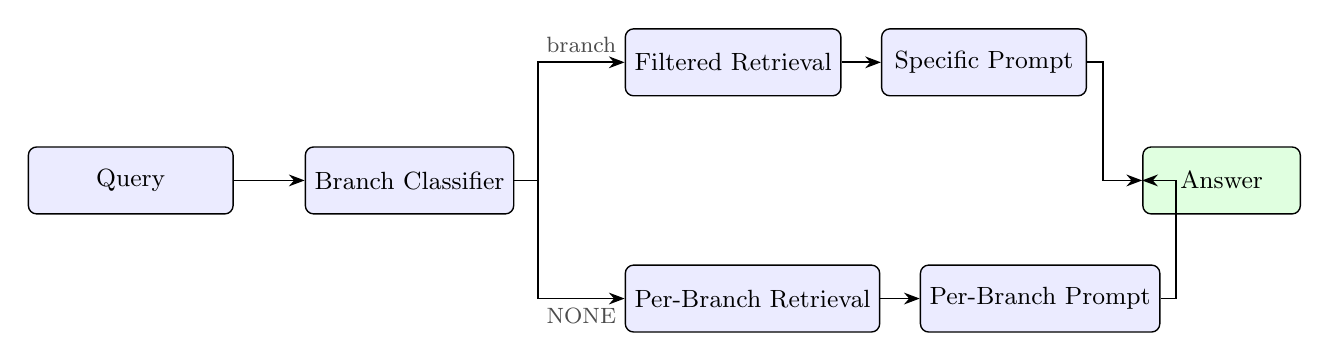
\begin{tikzpicture}[
  node distance=0.5cm and 0.5cm,
  box/.style={rectangle, draw, rounded corners=3pt, minimum height=0.85cm,
              minimum width=2.6cm, font=\small, align=center,
              fill=blue!8, line width=0.5pt},
  outbox/.style={rectangle, draw, rounded corners=3pt, minimum height=0.85cm,
              minimum width=2.0cm, font=\small, align=center,
              fill=green!12, line width=0.5pt},
  arrow/.style={-{Stealth[length=2mm]}, thick, line width=0.6pt},
  lbl/.style={font=\footnotesize, text=gray!60!black}
]
\node[box] (q) {Query};
\node[box, right=0.9cm of q] (cls) {Branch Classifier};
\node[box, right=1.4cm of cls, yshift=1.5cm] (top1) {Filtered Retrieval};
\node[box, right=0.5cm of top1] (top2) {Specific Prompt};
\node[box, right=1.4cm of cls, yshift=-1.5cm] (bot1) {Per-Branch Retrieval};
\node[box, right=0.5cm of bot1] (bot2) {Per-Branch Prompt};
\node[outbox, right=0.7cm of top2, yshift=-1.5cm] (a) {Answer};

\draw[arrow] (q) -- (cls);
\draw[arrow] (cls.east) -- ++(0.3,0) |- node[lbl, above, pos=0.75] {branch} (top1.west);
\draw[arrow] (cls.east) -- ++(0.3,0) |- node[lbl, below, pos=0.75] {NONE} (bot1.west);
\draw[arrow] (top1) -- (top2);
\draw[arrow] (bot1) -- (bot2);
\draw[arrow] (top2.east) -- ++(0.2,0) |- (a.west);
\draw[arrow] (bot2.east) -- ++(0.2,0) |- (a.west);
\end{tikzpicture}%
}
\caption{The canon-aware retrieval pipeline. The branch classifier routes the query either to filtered retrieval (when a branch is identified) or to per-branch retrieval (when no branch is identified). The seven evaluation configurations are toggles on this pipeline.}
\label{fig:arch}
\end{figure*}

\subsection{Corpus}

We construct a provenance-annotated corpus across three Stephen King works and their adaptations: \textit{The Shining} (novel 1977, Kubrick film 1980, 1997 miniseries), \textit{The Stand} (original 1978 edition, 1990 uncut edition, 1994 miniseries, 2020 miniseries), and \textit{Salem's Lot} (novel 1975, 1979 miniseries, 2004 miniseries, 2024 film). Eleven canon branches total.

Sources are secondary: Fandom wiki pages, Wikipedia plot summaries, and comparison articles from CBR, ScreenRant, SlashFilm, and Polygon. No primary novel or script text is used. Sources are fetched via the MediaWiki parse API for wikis and via direct HTML extraction for articles. Character pages with per-branch sections (e.g., Kurt Barlow) are split at the section level; pages without per-branch structure are retained under the novel branch only and noted as a limitation.

After deduplication, the corpus contains \textbf{436 chunks} with an average length of approximately 350 tokens. Chunk counts vary substantially across branches, ranging from 4 to 98 chunks.

\subsection{Seed Fact Table}

We manually construct a seed fact table of \textbf{43 verified canon conflicts}, each labeled with a work, event, branch, fact value, and conflict type (C1--C5). All facts are verified against the corpus. Facts where sources conflict irreconcilably are removed and recorded as a limitation.

\subsection{Query Set}

We generate \textbf{124 evaluation queries} from the seed fact table using an LLM-assisted pipeline, with manual verification against the corpus. Queries fall into four types:
\begin{itemize}
\item \textbf{EXPLICIT} (41): the query names a branch.
\item \textbf{IMPLICIT} (38): the query describes a branch without naming it.
\item \textbf{AMBIGUOUS} (24): the query names no branch and describes none.
\item \textbf{CONTROL} (21): the query has the same answer across all branches.
\end{itemize}

Ground truths for EXPLICIT and IMPLICIT queries are programmatically verified against the corpus via keyword matching, with manual review of flagged cases. AMBIGUOUS query ground truths list per-branch answers and are manually verified. CONTROL query ground truths are stable facts (character identities, authorship, stable plot elements).

\subsection{Inter-Annotator Agreement}

Two annotators independently labeled a stratified sample of 30 queries (10 EXPLICIT, 10 IMPLICIT, 10 AMBIGUOUS) into the four query types. Raw agreement was 90.0\% (27/30). Cohen's $\kappa$ was \textbf{0.850}, indicating almost perfect agreement. All disagreements occurred on queries where a branch was described by a distinctive trait without explicit naming (the IMPLICIT/AMBIGUOUS boundary).

\subsection{Retrieval Pipeline}

\textbf{Embeddings.} \texttt{BAAI/bge-small-en-v1.5}~\cite{bge}, normalized, cosine similarity.

\textbf{Vector store.} ChromaDB with metadata filtering on branch labels.

\textbf{Reranker.} \texttt{cross-encoder/ms-marco-MiniLM-L-6-v2}. Retrieval returns top-20; reranking returns top-5.

\textbf{Generator.} Groq's \texttt{openai/gpt-oss-120b}, temperature 0.0, max 1500 tokens.

\subsection{Variants}
\label{sec:variants}

We evaluate seven configurations. Each is a distinct point in the retrieval$\times$generation design space.

\textbf{Vanilla.} No branch awareness. Retrieval top-20, rerank top-5, standard generation prompt.

\textbf{B1 (Keyword filter).} A keyword dictionary maps surface tokens (``novel,'' ``1979,'' ``Kubrick'') to branch labels. If a keyword matches, retrieval is filtered to that branch; otherwise global retrieval. Standard generation prompt.

\textbf{B2 (Classifier filter).} An LLM classifies the query into one of the 11 branches or NONE. Filtered retrieval when a branch is identified; global retrieval otherwise. Standard generation prompt.

\textbf{Retrieval-only.} Per-branch retrieval for queries where the classifier returns NONE, but standard generation prompt. Isolates the retrieval contribution of per-branch retrieval.

\textbf{Prompt-only.} Global retrieval, but a per-branch generation prompt for queries where the classifier returns NONE. Isolates the generation contribution.

\textbf{B3 (Classifier + Per-Branch).} Combines retrieval-only and prompt-only: per-branch retrieval for unclassified queries, plus per-branch generation prompt.

The per-branch prompt instructs the generator to structure the answer as:
\begin{quote}
\small\ttfamily
The user did not specify a version. Answer for EACH version represented
in the context. Structure your answer as bullet points:
- In <version>: <answer>
If only one version appears in the context, say so explicitly.
Do not make up facts.
\end{quote}

\textbf{Universal-Prompt.} Global retrieval, but the per-branch generation prompt is applied universally to \emph{all} query types, regardless of whether the classifier found a branch. This isolates the effect of the prompt from the retrieval filtering.

\subsection{Answer-Level Evaluation}
\label{sec:judge}
Retrieval metrics measure whether retrieved chunks come from the expected branch. They do not measure whether the final answer is correct. To measure correctness, we use an LLM judge (\texttt{openai/gpt-oss-120b}, temperature 0.0) that scores each generated answer 0 or 1 against the ground truth:
\begin{itemize}
\item For EXPLICIT and IMPLICIT queries, the judge scores 1 if the answer contains the key fact from the ground truth, and 0 if it contradicts, omits, or fabricates facts.
\item For AMBIGUOUS queries, the judge scores 1 if the answer covers at least two versions and their respective outcomes, and 0 if it commits to one version only.
\item For CONTROL queries, the judge scores 1 if the answer contains the key fact.
\end{itemize}
The conflict-surfacing metric (ConflictSurf) reported in Table~\ref{tab:main} is a script-based keyword check that flags answers mentioning multiple distinct versions. It is distinct from the LLM judge's stricter AMBIGUOUS criterion, which additionally requires matching each version to its correct outcome.

\section{Results}

\subsection{Retrieval-Level Results}

Table~\ref{tab:main} reports retrieval precision (fraction of top-5 chunks from the expected branch, for EXPLICIT and IMPLICIT queries) and conflict surfacing (fraction of AMBIGUOUS queries where the answer mentions at least two distinct versions).

\begin{table}[htbp]
\caption{Retrieval-Level Results}
\begin{center}
\begin{tabular}{lccc}
\toprule
\textbf{Variant} & \textbf{EXPLICIT} & \textbf{IMPLICIT} & \textbf{AMBIGUOUS} \\
 & \textbf{RetrPrec} & \textbf{RetrPrec} & \textbf{ConflictSurf.} \\
\midrule
Vanilla & 0.46 & 0.41 & 16/24 \\
B1: Keyword & 0.54 & 0.39 & 19/24 \\
B2: Classifier & \textbf{0.98} & \textbf{0.54} & 13/24 \\
B3: Classifier + PB & 0.97 & 0.41 & \textbf{20/24} \\
\bottomrule
\end{tabular}
\label{tab:main}
\end{center}
\end{table}

\subsection{Answer-Level Results}
Table~\ref{tab:answer} reports answer-level correctness against ground truth, scored by an LLM judge (Section~\ref{sec:judge}). Figure~\ref{fig:answer_results} visualizes the same data as a heatmap.

\begin{table}[htbp]
\caption{Answer-Level Correctness}
\begin{center}
\begin{tabular}{lcccc}
\toprule
\textbf{Variant} & \textbf{EXPLICIT} & \textbf{IMPLICIT} & \textbf{AMBIG.} & \textbf{CONTROL} \\
\midrule
Vanilla & 21/41 & 29/38 & 12/24 & 20/21 \\
B1: Keyword & 11/41 & 30/38 & 15/24 & \textbf{21/21} \\
B2: Classifier & 20/41 & 24/38 & 12/24 & 19/21 \\
Retrieval-only & 20/41 & 23/38 & 16/24 & 20/21 \\
Prompt-only & 20/41 & 27/38 & 18/24 & 20/21 \\
B3: Classifier + PB & 20/41 & 27/38 & 19/24 & 20/21 \\
Universal Prompt & \textbf{24/41} & \textbf{31/38} & \textbf{20/24} & 20/21 \\
\bottomrule
\end{tabular}
\label{tab:answer}
\end{center}
\end{table}

\begin{figure}[t]
\centering
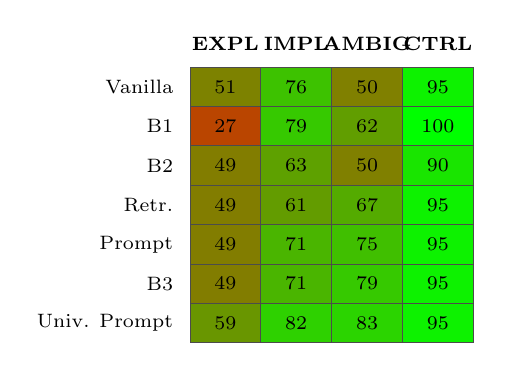
\begin{tikzpicture}[x=0.9cm, y=0.5cm]
  % Column headers
  \node[font=\scriptsize\bfseries] at (0.5, 0.6) {EXPL};
  \node[font=\scriptsize\bfseries] at (1.5, 0.6) {IMPL};
  \node[font=\scriptsize\bfseries] at (2.5, 0.6) {AMBIG};
  \node[font=\scriptsize\bfseries] at (3.5, 0.6) {CTRL};

  % Row labels
  \node[anchor=east, font=\scriptsize] at (-0.1, -0.5) {Vanilla};
  \node[anchor=east, font=\scriptsize] at (-0.1, -1.5) {B1};
  \node[anchor=east, font=\scriptsize] at (-0.1, -2.5) {B2};
  \node[anchor=east, font=\scriptsize] at (-0.1, -3.5) {Retr.};
  \node[anchor=east, font=\scriptsize] at (-0.1, -4.5) {Prompt};
  \node[anchor=east, font=\scriptsize] at (-0.1, -5.5) {B3};
  \node[anchor=east, font=\scriptsize] at (-0.1, -6.5) {Univ. Prompt};

  % Cells: x/row/value (percent)
  \foreach \x/\y/\v in {
    0/0/51, 1/0/76, 2/0/50, 3/0/95,
    0/1/27, 1/1/79, 2/1/62, 3/1/100,
    0/2/49, 1/2/63, 2/2/50, 3/2/90,
    0/3/49, 1/3/61, 2/3/67, 3/3/95,
    0/4/49, 1/4/71, 2/4/75, 3/4/95,
    0/5/49, 1/5/71, 2/5/79, 3/5/95,
    0/6/59, 1/6/82, 2/6/83, 3/6/95
  } {
    \pgfmathsetmacro{\rval}{int(100-\v)}
    \fill[red!\rval!green] (\x, -\y-1) rectangle (\x+1, -\y);
    \draw[black!70, line width=0.3pt] (\x, -\y-1) rectangle (\x+1, -\y);
    \node[font=\scriptsize] at (\x+0.5, -\y-0.5) {\v};
  }
\end{tikzpicture}
\caption{Answer-level correctness across seven configurations (percent correct). Cell color encodes rate: red = low, green = high. The EXPLICIT column shows branch-aware variants perform at or below vanilla, while keyword filtering (B1) is catastrophic. The AMBIGUOUS column shows that generation prompts produce the largest gains.}
\label{fig:answer_results}
\end{figure}

\subsection{Finding 1: Retrieval Precision Does Not Predict Answer Correctness}
\label{sec:finding1}

Compare Table~\ref{tab:main} to Table~\ref{tab:answer}. B2 raises EXPLICIT retrieval precision from 0.46 (Vanilla) to 0.98 --- nearly perfect. EXPLICIT answer correctness stays flat: 0.51 under Vanilla, 0.49 under B2. A variant that more than doubles the retrieval metric produces no improvement in end-to-end correctness, and in this case a marginal loss.

This is the paper's central empirical result. Retrieval precision is not a sufficient proxy for answer quality in provenance-aware systems.

\subsection{Finding 2: Keyword-Based Branch Filtering Halves Answer Correctness Despite Improving Retrieval Precision}

The divergence is more pronounced for B1. Keyword filtering raises EXPLICIT retrieval precision modestly (0.46 to 0.54), but EXPLICIT answer correctness collapses to 0.27 --- the worst of any configuration, and roughly half of Vanilla's 0.51. Because the keyword dictionary fires on surface tokens (``novel,'' ``book'') that appear across all three works, it frequently misroutes queries to the wrong branch. This misrouting leads to the lowest answer correctness among all configurations, despite the moderate retrieval precision.

B1 is a cautionary case: a variant can improve a standard retrieval metric while producing severe end-to-end degradation. Only answer-level measurement reveals the failure.

\subsection{Finding 3: Generation Prompts Outperform Retrieval Filtering}
\label{sec:finding3}

We isolate the contribution of the retrieval and generation components via the ablation in Table~\ref{tab:answer}. For AMBIGUOUS queries:

\begin{itemize}
\item B2 (no per-branch retrieval, no per-branch prompt): 12/24
\item Retrieval-only (per-branch retrieval, no per-branch prompt): 16/24
\item Prompt-only (no per-branch retrieval, per-branch prompt): 18/24
\item B3 (both): 19/24
\end{itemize}

Per-branch retrieval alone recovers 4 queries above B2. The per-branch prompt alone recovers 6. Both together recover 7. The prompt accounts for the majority of the improvement.

For IMPLICIT queries, the pattern is similar. Prompt-only recovers 27/38 (matching B3), while retrieval-only reaches only 23/38. The per-branch prompt is again the load-bearing component.

\subsection{Finding 4: A Universal Per-Branch Prompt Performs Best Under Lenient Evaluation}

To test whether the prompt's benefit extends beyond AMBIGUOUS queries, we introduced a universal-prompt configuration: global retrieval paired with the per-branch prompt applied universally to \emph{all} query types. 

This configuration achieves the highest raw scores on EXPLICIT (0.59), IMPLICIT (0.82), and AMBIGUOUS (0.83). However, we note a caveat for EXPLICIT queries. Because the universal prompt instructs the model to list all versions, and the judge rewards the presence of the correct fact, the model can score a 1 even if it also lists facts from other branches. This violates strict user-determined arbitration (failure mode F6: over-inclusion). The universal prompt's gain over Vanilla on EXPLICIT (+3 queries), where both use global retrieval, suggests that structuring the output may improve recall. However, this difference is within single-run noise. We leave a strict branch-fidelity metric to future work.

\subsection{Finding 5: In Our Setting, Generation-Side Changes Dominate}

Taken together, the results suggest that in our setting, the largest single contributor to provenance-aware correctness is the generation prompt, not the retrieval method. While the script-based ConflictSurf metric in Table~\ref{tab:main} detects keywords indicating multiple versions in 16/24 answers, the LLM judge scores Vanilla at only 12/24. This gap may reflect either that the generator fails to correctly pair outcomes with their respective versions, or that the judge is stricter than the keyword metric.

We note two caveats. First, this is an empirical observation from a single generator and a single run. Second, our per-branch prompt and our AMBIGUOUS judge both reward covering multiple versions. However, as discussed in Finding 4, while the universal prompt achieves the highest raw scores, the EXPLICIT gains may partially reflect the judge rewarding over-inclusion rather than strict adherence to user-specified provenance.

\subsection{Per-Branch Analysis}
\label{sec:perbranch}

The aggregate EXPLICIT precision of 0.46 (Vanilla) masks wide per-branch variation. Table~\ref{tab:perbranch} reports retrieval precision per branch, sorted by corpus size. Figure~\ref{fig:perbranch} visualizes the relationship between branch size and retrieval precision. We compare Vanilla and B2 as representative global and classifier-filtered retrieval modes.

\begin{table}[htbp]
\caption{Per-Branch Retrieval Precision}
\begin{center}
\begin{tabular}{lccccc}
\toprule
\textbf{Branch} & \textbf{Chunks} & \textbf{Queries} & \textbf{Van.} & \textbf{B2} & \textbf{$\Delta$} \\
\midrule
SHINING\_KUBRICK & 98 & 15 & 0.75 & 0.72 & $-0.03$ \\
STAND\_NOVEL\_1978 & 81 & 6 & 0.23 & 0.83 & $+0.60$ \\
SHINING\_NOVEL & 48 & 15 & 0.49 & 0.76 & $+0.27$ \\
SALEMS\_LOT\_NOVEL & 42 & 16 & 0.49 & 0.86 & $+0.37$ \\
STAND\_1994 & 32 & 2 & 0.60 & 1.00 & $+0.40$ \\
SALEMS\_LOT\_1979 & 24 & 7 & 0.29 & 0.77 & $+0.48$ \\
SHINING\_1997 & 14 & 2 & 0.20 & 1.00 & $+0.80$ \\
SALEMS\_LOT\_2004 & 12 & 7 & 0.14 & 0.57 & $+0.43$ \\
STAND\_2020 & 11 & 4 & 0.25 & 0.55 & $+0.30$ \\
STAND\_NOVEL\_1990 & 5 & 5 & 0.16 & 0.80 & $+0.64$ \\
\bottomrule
\end{tabular}
\label{tab:perbranch}
\end{center}
\end{table}

\begin{figure}[t]
\centering
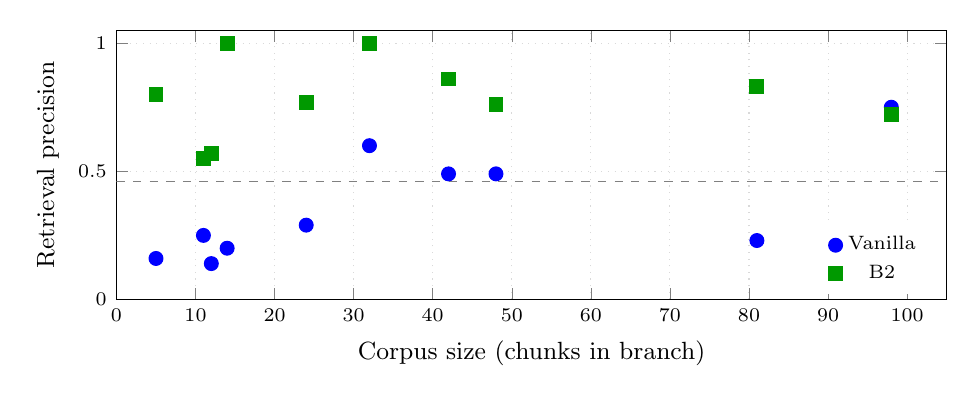
\begin{tikzpicture}
\begin{axis}[
  width=\columnwidth,
  height=5cm,
  xlabel={Corpus size (chunks in branch)},
  ylabel={Retrieval precision},
  xlabel style={font=\small},
  ylabel style={font=\small},
  xmin=0, xmax=105,
  ymin=0, ymax=1.05,
  grid=major,
  grid style={dotted, gray!30},
  legend style={at={(0.98,0.02)}, anchor=south east, font=\scriptsize, draw=none},
  tick label style={font=\scriptsize},
]
\addplot[only marks, mark=*, mark size=2.5pt, blue] coordinates {
  (98, 0.75) (81, 0.23) (48, 0.49) (42, 0.49) (32, 0.60)
  (24, 0.29) (14, 0.20) (12, 0.14) (11, 0.25) (5, 0.16)
};
\addplot[only marks, mark=square*, mark size=2.5pt, green!60!black] coordinates {
  (98, 0.72) (81, 0.83) (48, 0.76) (42, 0.86) (32, 1.00)
  (24, 0.77) (14, 1.00) (12, 0.57) (11, 0.55) (5, 0.80)
};
\addplot[domain=0:105, dashed, gray] coordinates {(0,0.46) (105,0.46)};
\legend{Vanilla, B2}
\end{axis}
\end{tikzpicture}
\caption{Retrieval precision versus corpus size per branch. Vanilla retrieval (blue) exhibits a dominance bias: thin branches receive low precision because dominant branches absorb the retrieval budget. B2 (green) corrects this for every branch except the largest (SHINING\_KUBRICK), which vanilla already over-represents.}
\label{fig:perbranch}
\end{figure}

We identify a \emph{dominance bias} in vanilla retrieval. Branches with more chunks about a query topic dominate retrieval regardless of the branch the user asked about. STAND\_NOVEL\_1978 (81 chunks, second largest) achieves only 0.23 precision in vanilla because comparison-article chunks covering the same topics dominate retrieval. SALEMS\_LOT\_2004 achieves 0.14; STAND\_NOVEL\_1990 achieves 0.16.

Branch classification (B2) corrects this for every under-represented branch. Gains range from $+0.27$ to $+0.80$. However, the effect is not uniform. SHINING\_KUBRICK (98 chunks, largest branch) shows no improvement (0.75 to 0.72), because vanilla retrieval already over-represents it. Branch-aware retrieval is therefore most valuable for branches that are under-represented relative to the dominant branch, not uniformly across branches.

This per-branch analysis is essential for interpreting the aggregate metrics. The improvement in aggregate EXPLICIT precision from 0.46 to 0.98 is largely attributable to correcting the dominance bias. However, as shown in Section~\ref{sec:finding1}, this correction does not propagate to answer correctness.

\subsection{Case Studies}
\label{sec:casestudies}

We trace five queries across the vanilla baseline and the branch-aware variants to illustrate the failure modes and the improvements the variants introduce.

\textbf{Case 1: Silent resolution on an ambiguous query (Q019).} Query: ``How does Jack Torrance die?'' (AMBIGUOUS). Vanilla retrieved mixed branches and answered with the novel's boiler explosion as fact, without acknowledging the Kubrick film's freezing death. This is failure mode F3 (silent resolution). B3 answered with both versions in a structured list.


\textbf{Case 2: Retrieval contamination despite correct classification (Q017).} Query: ``How does Jack Torrance die in the novel of The Shining?'' (EXPLICIT, expected branch SHINING\_NOVEL). B2 correctly classified the query as SHINING\_NOVEL, but the chunk that states the novel's ending is located on a Kubrick wiki page that describes the film's divergence from the novel. That chunk is labeled SHINING\_KUBRICK and was excluded by the branch filter. The answer omits the correct fact. This case illustrates a limitation of metadata-only branch filtering.

\textbf{Case 3: Per-branch dilution on an implicit query (Q086).} Query: ``What happens to Susan when Ben intends to save her rather than destroy her?'' (IMPLICIT, expected branch SALEMS\_LOT\_2004). The query describes a distinctive 2004 plot event without naming it. Under B2, the classifier returned SALEMS\_LOT\_2004 and retrieval was filtered accordingly. Under B3, the same classifier returned NONE, triggering the per-branch fallback; top-3 chunks from every branch diluted the SALEMS\_LOT\_2004 results. This case illustrates the explicit/implicit trade-off quantified in Table~\ref{tab:main} (IMPLICIT precision 0.54 for B2 vs 0.41 for B3).

\textbf{Case 4: Full variant trace on a single query (Q005).} Query: ``Does Dick Hallorann survive The Shining?'' (AMBIGUOUS). Ground truth: Hallorann survives in the novel and the 1997 miniseries; he dies in the 1980 Kubrick film.

\emph{Vanilla.} Top-5 retrieval returned three SHINING\_KUBRICK chunks, two SHINING\_NOVEL chunks, and no SHINING\_1997 chunks. The answer reported that Hallorann survives, citing only novel context and never mentioning that the Kubrick film diverges. The information about Kubrick's version was in the context window and the generator ignored it. This is failure mode F3.

\emph{B2 (Classifier).} The classifier returned SHINING\_KUBRICK. Retrieval was filtered to that branch and all five chunks came from the film corpus. The answer reported that Hallorann is killed by Jack, without acknowledging any other version. The classifier over-committed on an ambiguous query, and the answer became \emph{less} correct than vanilla's.

\emph{Prompt-only.} Retrieval was global (same as Vanilla), but the per-branch prompt was used. The generator produced a structured answer listing SHINING\_NOVEL (survives), SHINING\_KUBRICK (dies), and SHINING\_1997 (survives). The conflict was surfaced using the same retrieval as Vanilla, purely by changing the prompt. This demonstrates that the prompt can surface conflicts even with unfiltered retrieval.

\emph{B3 (Classifier + Per-Branch).} The classifier again returned NONE, triggering per-branch retrieval. The answer was substantially identical to Prompt-only's --- the same three-branch structure --- confirming that the retrieval change added little.

\section{Error Analysis}

We categorize observed failures into six types, extended from our conflict taxonomy:

\begin{itemize}
\item \textbf{F1: Canon mixing.} The answer combines facts from multiple branches without acknowledgment.
\item \textbf{F2: Branch misidentification.} The answer uses the wrong branch for an EXPLICIT query.
\item \textbf{F3: Silent resolution.} The answer picks one branch for an AMBIGUOUS query without surfacing the conflict.
\item \textbf{F4: Cross-work conflation.} The answer merges facts from two unrelated works.
\item \textbf{F5: Fabrication.} The answer asserts a fact not present in any branch.
\item \textbf{F6: Over-inclusion.} The answer lists facts from multiple branches even when the user specified a single branch.
\end{itemize}

Additional failure modes observed:

\textbf{Empty responses.} The generator (a reasoning model) exhausted its token budget on internal reasoning, producing no output. We count these as incorrect.

\textbf{Spurious citation markers.} The generator occasionally appended markers such as bracketed source references that do not correspond to source chunks. These did not affect answer correctness but indicate formatting instability.

\textbf{Retrieval contamination.} Chunks labeled for one branch often describe another, particularly in comparison articles and wiki pages that discuss multiple versions. This limits the effectiveness of metadata-only branch filtering, and is a root cause of the Case 2 failure.

\section{Threats to Validity}

\subsection{Internal Validity}

The reported retrieval precision measures whether retrieved chunks come from the expected branch. It does not measure whether those chunks contain the answer. A chunk from the correct branch may not contain the relevant fact (Case 2 in Section~\ref{sec:casestudies}), and a chunk from the wrong branch may.

Per-branch sample sizes are uneven. Some branches (SHINING\_KUBRICK, SHINING\_NOVEL, SALEMS\_LOT\_NOVEL) are represented by 15 to 16 queries each; others (STAND\_1994, SHINING\_1997) by only 2. Aggregate metrics are dominated by the larger branches, and per-branch deltas for small branches should be treated as preliminary.

Inter-annotator agreement was computed on 30 queries. The disagreements we observed ($\kappa = 0.85$, three disagreements out of 30) all fell on the IMPLICIT/AMBIGUOUS boundary.

The LLM judge was validated on a stratified sample of 40 judged answers (10 per query type) hand-labeled by the first author. Overall agreement was 35/40 (87.5\%). Agreement was highest on CONTROL (100\%) and AMBIGUOUS (90\%) queries, and lowest on EXPLICIT queries (70\%). Disagreements primarily occurred because the judge was overly strict on EXPLICIT answers, penalizing semantically correct answers for not matching the exact phrasing of the ground truth. Consequently, the EXPLICIT comparisons (e.g., B2's 20/41 vs Vanilla's 21/41) are subject to noise and should not be over-interpreted. However, the AMBIGUOUS comparisons (where agreement was 90\%) carry our headline results and are more reliable, though we note that 90\% agreement indicates the judge reliably counts versions, not necessarily that the metric fully captures arbitration quality.

The generator is non-deterministic at the token level. We did not run repeated trials; the reported results are from a single run per variant. The ablation comparisons in Section~\ref{sec:finding3} involve one-query differences between Prompt-only and B3; those should be treated as suggestive rather than confirmatory.

\subsection{External Validity}

We evaluate on three Stephen King works. All three have well-known adaptations, active fan communities, and substantial secondary literature. Whether the findings transfer to franchises with different adaptation structures or to works with no public wiki is a hypothesis, not a demonstrated result.

Whether the findings transfer to non-fiction parallel-source domains (legal jurisdictions, medical guidelines, historical disputes) is also a hypothesis. These domains share the structural property of parallel valid sources, but sources are often hierarchically ordered by jurisdiction or recency, and users may not know which source is authoritative. Fiction canon is a clean test case precisely because no universal hierarchy exists.

The corpus is small (436 chunks) relative to production RAG systems. Retrieval behavior at scale may differ.

\subsection{Construct Validity}

``Canon branch'' is an operational definition. We assign each chunk a single branch label based on its source file, but chunks often describe multiple versions. Our definition excludes chunks from a branch's retrieval pool even when they contain that branch's facts. This affects all variants and is the root cause of the case study failure in Section~\ref{sec:casestudies}.

The conflict taxonomy (C1--C5) is manual and may not capture all dimensions of canon conflict. The query type taxonomy was validated by inter-annotator agreement of $\kappa = 0.85$. The remaining disagreement concentrates on the IMPLICIT/AMBIGUOUS boundary, suggesting that these two categories may not be fully separable in practice.

\subsection{Conclusion Validity}

The main comparisons --- Vanilla vs. B2 on EXPLICIT, Universal-prompt vs. Vanilla on AMBIGUOUS --- are based on $N = 41$ and $N = 24$ respectively. An exact McNemar test on the per-query results indicates that we could not detect a significant difference between Vanilla and B2 on EXPLICIT answer correctness ($p = 1.000$); 13 of 41 answers flipped, with gains and losses offsetting. Conversely, the universal prompt's improvement over Vanilla on AMBIGUOUS queries is statistically significant ($p = 0.0078$), though this partly reflects the prompt's alignment with what the judge evaluates.

The IMPLICIT comparison between B2 and Prompt-only is based on $N = 38$ and represents a difference of 3 queries. This should be treated as suggestive rather than confirmatory.

The central empirical claim of the paper --- that retrieval precision does not predict answer correctness --- rests on the consistent pattern across four query types and seven configurations rather than on any single comparison. For example, B2 raises IMPLICIT retrieval precision from 0.41 to 0.54, yet answer correctness falls from 29/38 to 24/38. This divergence appears in a query type where the judge was highly reliable (90\% agreement).

\section{Reproducibility and Ethics}

\textbf{Code and data.} All scraping scripts, chunking scripts, retrieval pipelines, evaluation scripts, and scoring scripts are publicly available at \url{https://github.com/hvocr/canon-aware-rag}. The repository includes the corpus construction pipeline, the seed fact table, the 124-query evaluation set, the seven configuration runners, and the LLM-judge scoring scripts. Fandom wiki content is used under CC-BY-SA; Wikipedia content under CC-BY-SA. We do not redistribute primary novel or screenplay text.

\textbf{Human subjects.} This work does not involve human subjects. The inter-annotator agreement study used two annotators (one author and one volunteer) on publicly available queries; no personal data was collected.

\textbf{Compute.} All experiments ran on a single consumer laptop with an NVIDIA GTX 1650 Ti GPU (4~GB VRAM) and a free-tier API. No proprietary compute was used.

\section{Limitations}

\textbf{Single generator.} Results are from a single generator (\texttt{openai/gpt-oss-120b}). Whether the universal-prompt finding transfers to other models is untested. Smaller or larger models may show different failure profiles.

\textbf{Corpus contamination.} Sources that describe multiple versions label chunks with a single branch even when content spans branches.

\textbf{Annotation sample size.} Inter-annotator agreement was computed on 30 queries.

\textbf{Domain specificity.} We evaluate on Stephen King adaptations only. Generalization to other franchises and to non-fiction parallel-source domains is a hypothesis.

\textbf{Single run per configuration.} We did not repeat the ablation with different random seeds. The Prompt-only versus B3 difference of one query is within run-to-run noise.

\section{Conclusion}

We introduced user-determined provenance arbitration as a distinct problem from the conflict resolution studied in prior RAG work. We constructed a provenance-annotated benchmark of 43 canon conflicts and 124 queries across three Stephen King works, and evaluated seven retrieval-and-generation configurations at both retrieval and answer levels.

The two metrics diverge. Branch-aware retrieval nearly eliminates cross-branch retrieval for explicit queries (0.46 to 0.98 retrieval precision) but produces no improvement in answer correctness (0.51 to 0.49). Keyword-based branch filtering improves a retrieval metric while halving answer correctness (0.51 to 0.27). A universal per-branch generation prompt achieves the highest raw correctness scores (0.59 EXPLICIT, 0.82 IMPLICIT, 0.83 AMBIGUOUS). However, because our evaluation judge rewards the presence of the correct fact even when other branches are listed, we cannot claim this configuration fully respects user-determined arbitration.

The paper's central empirical claim is that branch-label retrieval precision does not predict answer-level correctness in our setting. We report this from a single-generator, single-run experiment. While a universal prompt achieves higher raw scores, it may not strictly respect user-specified provenance, highlighting the need for future evaluation metrics that explicitly penalize cross-branch mixing.

Future work should investigate generation protocols for provenance arbitration. A promising direction is a two-stage architecture that first classifies whether the query is provenance-specified, then selects between a specific and a per-branch generation mode. Such an architecture would formalize the trade-off we observe between explicit and ambiguous queries, and would treat the ambiguous case as a distinct generation task rather than a fallback. The benchmark, evaluation scripts, and configuration comparison are released to support this line of work.

\begin{thebibliography}{00}

\bibitem{lewis2020} P. Lewis et al., ``Retrieval-Augmented Generation for Knowledge-Intensive NLP Tasks,'' in \textit{Proc. NeurIPS}, vol. 33, pp. 9459--9474, 2020.

\bibitem{conflictrag} C. Wang, Y. Li, Y. Liu, and Y. Shu, ``ConflictRAG: Detecting and Resolving Knowledge Conflicts in Retrieval-Augmented Generation,'' arXiv:2605.17301, 2026.

\bibitem{truthfulrag} S. Liu, Y. Shang, and X. Zhang, ``TruthfulRAG: Resolving Factual-level Conflicts in Retrieval-Augmented Generation with Knowledge Graphs,'' in \textit{Proc. AAAI}, vol. 40, no. 38, pp. 32168--32176, 2026, doi:10.1609/aaai.v40i38.40489.

\bibitem{tgrag} D. Li et al., ``T-GRAG: A Dynamic GraphRAG Framework for Resolving Temporal Conflicts and Redundancy in Knowledge Retrieval,'' arXiv:2508.01680, 2025.

\bibitem{conrag} X. Sun, J. Chen, B. Zhou, and M.-J. Kuo, ``ConRAG: Contradiction-Aware Retrieval-Augmented Generation under Multi-Source Conflicting Evidence,'' \textit{Journal of Advanced Computing Systems}, vol. 4, no. 7, pp. 50--64, Jul. 2024, doi:10.69987/JACS.2024.40705.

\bibitem{authoritybias} Y. Li et al., ``LLMs Trust Humans More, That's a Problem! Unveiling and Mitigating the Authority Bias in Retrieval-Augmented Generation,'' in \textit{Proc. ACL}, 2025, pp. 28844--28858.

\bibitem{magic} J. Lee, L. Kangmin, and T. Kim, ``MAGIC: A Multi-Hop and Graph-Based Benchmark for Inter-Context Conflicts in Retrieval-Augmented Generation,'' in \textit{Findings of EMNLP}, 2025, pp. 8783--8803.

\bibitem{confact} Z. Ge et al., ``Resolving Conflicting Evidence in Automated Fact-Checking: A Study on Retrieval-Augmented LLMs,'' in \textit{Proc. IJCAI}, 2025, pp. 9656--9664.

\bibitem{nkw} Q. Tian et al., ``Narrative Knowledge Weaver: Narrative-Centric Retrieval-Augmented Reasoning for Long-Form Text Understanding,'' arXiv:2606.05724, 2026.

\bibitem{bge} S. Xiao, Z. Liu, P. Zhang, N. Muennighoff, D. Lian, and J.-Y. Nie, ``C-Pack: Packed Resources for General Chinese Embeddings,'' in \textit{Proc. SIGIR}, 2024. (Model: BAAI/bge-small-en-v1.5.)

\end{thebibliography}

\end{document}